\documentclass[Royal,times,sageh]{sagej}

\usepackage{moreverb,url,natbib, multirow, tabularx}
\usepackage[colorlinks,bookmarksopen,bookmarksnumbered,citecolor=red,urlcolor=red]{hyperref}



% tightlist command for lists without linebreak
\providecommand{\tightlist}{%
  \setlength{\itemsep}{0pt}\setlength{\parskip}{0pt}}



\usepackage{setspace}
\usepackage{float}
\floatplacement{figure}{H}


\begin{document}


\setcitestyle{aysep={,}}

\title{Congre(ss)gation: A Social Network Analysis of Religion and
Cosponsorship in the United}

\runninghead{Dionne \& Liftman.}

\author{Natalie Dionne\affilnum{1}, Naomi Liftman\affilnum{2}}

\affiliation{\affilnum{1}{Department of Government, Smith College,
Northampton, United States}\\\affilnum{2}{Department of Statistical and
Data Science, Smith College, Northampton, United States}}

\corrauth{Naomi Liftman}

\email{\href{mailto:naomiliftman@icloud.com}{\nolinkurl{naomiliftman@icloud.com}}}

\begin{abstract}
Given religion's recent influence on political decisions, we explore its
effect on legislative behavior in the United States Congress. We apply a
network analysis to all 70,000 pieces of cosponsored legislation from
both the 112th and the 117th Congresses to infer a series of political
relationships among legislators. From this network we test (1) if
religion influences cosponsorship in the congressional network, and (2)
if that influence has changed in the last ten years. We find evidence
that religious identity has affected legislators' cosponsorship behavior
in recent years, but not in the past. This analysis suggests an increase
in religion-based polarization in the United States Congress.
\end{abstract}

\keywords{Cosponsorship, Congressional Networks, Religion, Religious
Identity, Polarization}

\maketitle

\singlespacing

\hypertarget{introduction}{%
\section{Introduction}\label{introduction}}

\doublespacing

~~The very first words of the United States Bill of Rights attempt to
draw a line between religion and politics. At that time most Americans
agreed with the statement that Congress should make ``no law respecting
an establishment of religion or prohibiting its free exercise
\citeyearpar{billrights}''. However, the recent threat to the domination
of Christian ideology has prompted a Republican push to factor religion
into political decisions. In the last year, the conservative Supreme
Court, on multiple occasions, has ruled in favor of Christians and
Christians organizations \citep{bum2023}. As we enter a post-roe
America, we must understand the depths of religious influence in our
politics. Is church still separate from state? Has our congress become a
congregation?

We look to study the relationship between religious identity and
cosponsorship networks in the United States Congress. Extensive
literature supports the importance of cosponsorship as the core activity
in building the legislative agenda. As Schiller
\citeyearpar{schiller1995} demonstrates, sponsorship and cosponsorship
are two of the few legislative activities members of Congress have
almost total control over. Member's can decide to introduce and support
legislation that appeases their constituents, progresses their political
career, and initiates institutional change on a variety of policies.
While legislators, as individuals, sponsor and cosponsoring bills,
scholarship argues a cosponsorship approach is the best method to infer
which legislators support which legislatures \citep{fowler2006}. With
that, cosponsorship has become the most used tie when modeling the
social network of congress.

A growing body of literature explores the effects of a variety of
identity-based characteristics on cosponsorship networks in the
legislative body. This research has focused primarily on basic political
identities (i.e., partisanship, political ideology, and district
representation) and visible identity characteristics (i.e., race,
gender, and ethnicity). Both have provided extensive support for
Huckfeldt's \citeyearpar{huckfeldt1983} claim that one's community and
individual characteristics influence their political actions. Existing
research has also found evidence for the psychological theory of Social
Identity \citep{tajfel}, which argues that individuals, especially
minority groups, favor those within their own identity-based
communities.

However, existing scholarship on identity does not contain research on
the effect of religious affiliation in the congressional cosponsorship
network. Given religion's intrinsic function as a core component of an
individual's identity and its known effect on political ideology
\citep{mctague}, there is a skeleton framework that religion influences
legislators' actions. Thus this paper provides empirical evidence for
the legislators' religious identity affects the congressional
cosponsorship network.

In this paper, we examine religious identity among two Congresses: the
United States 112th and the 117th . Data on sponsorship and
cosponsorship is used in conjunction with network analysis to model the
influence of religion in each session. We then compare the resulting
networks to understand how the effect of religious affiliation on
congressional ties has changed over the ten years studied. With this, we
find evidence that religious identities' effects cosponsorship in the
117th Congress, but not the 112th, both in general and also when
in-group homophily is explored. This directly contributes to the
existing body of literature on recent trends in polarization,
specifically the growing political division created by religious
differences.

\hypertarget{congressional-cosponsorship-networks}{%
\subsection{Congressional Cosponsorship
Networks}\label{congressional-cosponsorship-networks}}

~~Cosponsorship has become the most common strategy for indirectly
inferring legislators' relations and has been used to examine state and
federal bodies globally \citep{neal2020}. Schiller
\citeyearpar{schiller1995} argues that bill sponsorship is one of the
few activities over which legislators have almost total control. Thus,
it is the means by which legislators can introduce and support
legislation that appeases their constituents, progresses their political
career, and enacts change in a variety of areas. The bill sponsorship
system in the United States is designed with one ``primary sponsor,''
which is the legislator who introduces the bill and any number of
``cosponsors,'' who also support the bill but are not responsible for
drafting. Although, some bills are coauthored, there is only one formal
primary sponsor; the rest of the legislators who sign their support to
the bill are cosponsors.

While legislatures can be thought of as individually sponsoring and
cosponsoring data, studies have found that the activity of cosponsorship
within when examined as a whole is more reflective of network
involvement \citep{fowler2006}. Existing scholarship further defends the
idea of legislative power of cosponsorship through its ability to set
the agenda. Agenda-setting is the process by which policymakers
effectively control or manage the issues that receive political
attention. While most bills do not pass and less than 4\% receive
cosponsors, the sponsorship process determines what issues are on the
table and, therefore, subject to institutional change
\citep{bratton2011}.

Using cosponsorship data as a tie to connect legislators in the
congressional network was largely pioneered by Fowler
\citeyearpar{fowler2006} when he discovered that analysis normally
focuses on which bills legislators will support rather than which
legislators will support other legislators. He then used social network
analysis to examine cosponsorship from 1973 to 2004 in the United States
Congress. Crafting a measure of connectedness, he found that
well-connected legislators are more successful at passing amendments and
gaining support in roll-call votes, a frequent indicator of political
influence.

\hypertarget{identity-based-congressional-cosponsorship-networks}{%
\subsection{Identity-Based Congressional Cosponsorship
Networks}\label{identity-based-congressional-cosponsorship-networks}}

~~There is also a growing body of evidence that core characteristics of
a legislator's identity have an effect on the congressional network.
This tendency, ``often described as `birds of a feather flock together,'
is prevalent across social networks in a variety of contexts, from
friendship groups to schools and businesses'', creating a strong
likelihood of its prevalence in Congress \citep[pg. 2]{craig2015}. This
connection to the congressional network began with Huckfeldt
\citeyearpar{huckfeldt1983}, who originally theorized that one's
community and individual characteristics influence how they interact in
the political sphere. This laid the foundation for an investigation into
the effects of race, gender, and ethnic identity on cosponsorship in the
congressional network.

\hypertarget{political-identity-based-congressional-cosponsorship-networks}{%
\subsubsection{Political Identity-Based Congressional Cosponsorship
Networks}\label{political-identity-based-congressional-cosponsorship-networks}}

~~Research using congressional cosponsorship data has identified that,
first and foremost, social networks are affected by basic similarities
and political identities. Using a multi-level network approach, Gross
\citeyearpar{gross2007} discovered that shared committee service,
similarity in ideology, and being elected from the same state or region
are all factors that contribute to cosponsorship. Meanwhile, Zhang et
al. \citeyearpar{zhang2007} concluded that cosponsorship networks are
influenced by ideology, committee service, and geography. Furthermore
Caldeira and Patterson's \citeyearpar{caldeira} findings indicate that
legislative relationships are influenced by both propinquity, which
refers to the distance between districts or seatmates, and shared
characteristics such as similar levels of education, party affiliation,
and shared committee assignments.

This body of literature defends the idea that basic similarities, such
as being from the state or of the same age, as well as core political
components of identity (often job related) affect congressional
cosponsorship behavior. Bratton and Rouse's \citeyearpar{bratton2011}
research reinforces these claims in the validation of their first
hypothesis, which provides sufficient evidence that legislatures are
more likely to cosponsor measure if those legislators are similar in
some significant ways, such as shared background experiences, political
interests, or ideological predispositions.

\hypertarget{visible-identity-based-congressional-cosponsorship-networks}{%
\subsubsection{Visible Identity-Based Congressional Cosponsorship
Networks}\label{visible-identity-based-congressional-cosponsorship-networks}}

~~While there is a growing body of literature on the effects of
homophily (similar visible identity characteristics such as race,
gender, and ethnicity), it is far more split than the research regarding
the basic components of political identity. For example, Bratton and
Rouse \citeyearpar{bratton2011} examine numerous social determinants
within the cosponsorship network of state legislators. However, their
conclusions on the effects of gender and race on legislators' general
propensity to cosponsor varied by state. They found strong correlations
between homophily and cosponsorship in Texas and California but moderate
effects in the other states of interest. Yet, when they factored
minority status into the equation, they found a strong correlation in
every state legislature. This means that women, Latino people, and
African-American people were relatively more likely to endorse the
proposals of others who shared their respective minority status. While
they can only hypothesize, Bratton and Rouse \citeyearpar{bratton2011}
suggest the distinction is due to the social identity theory.

Social identity theory is a psychological concept that provides insight
into the characteristics of group boundaries and behavior. At its core,
social identity theory argues that a person's sense of self comes from
their group memberships. The founder of the theory, Tajfel
\citeyearpar{tajfel}, found that the process of categorizing oneself as
a group member creates a positively valued social identity. Once
allegiances have been set, individuals will allocate more resources to
the in-group to maximize their benefits over the out-group.
Psychologists in the years since have discovered this to be especially
true as it relates to minority groups - women, Latino, and
African-American legislators \citep{huddy2004}. Due to the systematic
disadvantages these individuals face, they are more likely to support
those within their respective social group over others. While majority
group members have the potential to display bias towards their in-group,
the effect of a minority identity-based characteristic is more likely to
be seen.

As it relates to women, Barnes \citeyearpar{barnes2015} examined the
structure of the legislature to see if women are excluded from the
``men's club.'' In doing so, Barnes provides extensive background on
what encourages women to collaborate in the political sphere. Her
analysis provides evidence that women are relatively more likely to
cosponsor measures introduced by other women. Wojcik and Mullenax
\citeyearpar{wojcik}, using survey-based evidence from Brazil's Chamber
of Deputies, argue that female representatives engage in higher rates of
intragender networking. This means women have more profuse and diverse
legislative networks than male representatives. Together, these findings
support the idea that networks are affected by gender identity.
Specifically, this provides evidence for in-group favoritism within the
gender minority, which supports the psychological claims about the
effects of minority identity-based characteristics.

Rocca and Sanchez \citeyearpar{rocca} support similar conclusions
regarding the effects of identity on the network, as it relates to
minority racial and ethnic groups. They find that, on average, Black and
Latino legislators sponsor and cosponsor significantly fewer bills in
Congress than Whites and non-Latinos, respectively. Black and Latino
legislatures prioritize sponsoring each other's legislation. Rocca and
Sanchez \citeyearpar{rocca} attribute this conclusion to the components
of the social identity theory, specifically the systematic disadvantages
in access to resources and the resulting desire to support one's own
group. Craig et al. \citeyearpar{craig2015} study the U.S. House
cosponsorship network from 1981 through 2004 to highlight the ways in
which visible identity characteristics have circumscribed the minority
experience. They find that Black and Latino members of Congress are at a
comparative disadvantage of race-based assortative mixing in the
cosponsorship process. This literature not only supports the idea that
race and ethnic identity affect the congressional cosponsorship network
but provides more framework for distinguishing on majority / minority
lines.

\hypertarget{religious-identity}{%
\subsection{Religious Identity}\label{religious-identity}}

~~The literature on the congressional cosponsorship networks is vast.
Studies regarding the effects of basic (and political) similarities, as
well as gender, race, and ethnicity are becoming increasingly abundant.
However, quite surprisingly, there is little (if any) research on how
religion influences the congressional cosponsorship network.

Religion is a core component of a legislature's identity, for some as
intrinsic as their sex or race, and for others entirely intertwined with
their ideology. Given this nature, we should expect a legislator's
religious affiliation to have a significant effect on their political
decision. Research has shown it does. Mctague \& Pearson-Merowitz
\citeyearpar{mctague} highlight how religious affiliation can predict
party affiliation (with Jews representing the most liberal, Catholics
and Protestants representing the moderate, and evangelical Christians
representing the furthest right). They also explain that the recent
growth in partisan polarization over cultural and ideological issues
only increases the tendency to follow one's religion to a political
party. Religion is, therefore, an intrinsic identity that divides
individuals into an in-group and an out-group. This provides evidence
that religion has the potential to function exactly like sex, race, and
ethnicity.

With that, we have created two hypotheses to fill the gap in the
literature on religion within the congressional cosponsorship network.

\emph{H1: (general) Legislators will be more likely to cosponsor
measures sponsored by colleagues with the same religious affiliation.}

\emph{H2: (minority group) Those belonging to religious minority groups
will be relatively more likely to cosponsor measures introduced by
another member of the same religious minority (i.e., Jewish legislators
will be more likely to cosponsor bills introduced by other Jewish
legislators)}

\hypertarget{trends-over-time-polarization}{%
\subsection{Trends Over Time:
Polarization}\label{trends-over-time-polarization}}

~~Social Network Analysis, specifically using cosponsorship as a tie,
has long examined cooperation among congressional representatives. As
previously explained, modeling the network in this manner, allows for
extensive research on the effects of a variety of different identities.
Typically this is taken one step further to account for change overtime.
When the legislative network is examined in this manner, researchers are
able to better understand and qualify the growing polarization in
congress over the past decade.

In the United States' two-party system polarization is commonly seen in
the growing distinction between the Republican and Democratic parties.
However, in its most basic form polarization simply refers to the sharp
contrast between two different ideas or set beliefs. Working off of that
definition, polarization can be seen in a variety of contexts including
gender, ethnicity, and media. Using components of the Social Identity
Theory, Neal \citeyearpar{neal2020} distinguishes between weak and
strong polarization to provide a foundational understanding of the
concept. Weak polarization refers to very high rates of in-group support
with low or non-existent out-group relations. This, as he defines it, is
categorized by indifference rather than active animosity towards those
in other communities. Strong polarization, on the other hand, is the
presence of negative relations between the two polarized groups.
Research has shown that strong polarization is steadily increasing in
Congress and deeply affects legislators ability to introduce and pass
legislation. Using a time based approach, cosponsorship networks have
been able to show that legislators are more likely to support those
with-in their group and oppose those outside. Ultimately, polarization
is a growing and active problem within the congressional network.

With that, we have created our last hypotheses to understand if religion
is contributing to the growing polarization within the congressional
cosponsorship network.

\emph{H3: (increased polarization) There will be a stronger effect of
religion in the 117th Congress compared to the 112th Congress (measured
by legislators being more likely to cosponsor measures sponsored by
colleagues with the same religious affiliations).}

\hypertarget{research-design}{%
\section{Research Design}\label{research-design}}

~~To measure positive relationships between legislators we used a
cosponsorship network for the 112th and 117th Congress's separately. In
each session we built a network with legislators as the nodes and the
edges being the `level of cosponsorship' which is measured as the total
number of times legislator \(A\) cosponsors legislator \(B\)'s
legislation divided by the average number of cosponsorship between
legislators per session. This tie is directional as cosponsoring
legislator \(B\)'s bill is a sign of support from legislator \(A\) which
may not inherently be reciprocated. Thus the cosponsorship network is
directed, weighted, and excludes self-ties. In both the 112th and 117th
networks we include three edge level covariables: religion, ideology,
and party. Religion and party are binary, undirected, and exclude
self-ties, with Ideology being weighted, undirected, and excluding
self-ties.

In order to assess the effects of religious affiliation over time, we
look at the 112th and 117th Congress'. These Congresses were chosen
because the 112th ran from January 3, 2011 to January 3, 2013, which was
after the 2008 financial crisis and before the election of Donald Trump.
Thus, this Congress acts as a `control' case for how religious
affiliation affects cosponsorship. The 117th Congress was chosen as it
is the most recent congress to finish a full session running from
January 3, 2021 to January 3, 2023. Thus at the time of writing this
Congress was recently completed and is the most current Congress with
cosponsorship data available. These sessions are also direct mirrors of
each other with the 112th having a Democratic President and Senate with
a Republican House and the 117th having a Republican President and
Senate and a Democratic House.

There are three sets of models used to assess the effect of religious
affiliation on cosponsorship. Each model was run for the 112th and 117th
session separately. The first set of models assess' the general and
polarization hypotheses using network regression:

\(cosponsorship = B_1(religion) + B_2(party) + B_3(ideology)\),

and we expect religion to be statistically significant for the 117th
congress but not the 112th Congress due to an increase in polarization.
We do not expect party or ideology to be statistically significant, as
they are control variables to mitigate covariance.

The second set of models assess the minority group and polarization
hypotheses using another network regression model:

\(cosponsorship = B_1(catholic) + B_2(jewish) + B_3(other) + B_4(protestant) + B_5(unknown)\),

and we expect Jewish and Other to be statistically significant in both
the 112th and 117th Congress' in congruence with previous literature on
minority group activity. We will also expect more religious affiliation
groups to be statistically significant in the 117th compared to the
112th due to recent polarization. The final set of models are similar to
the second set, except include ideology and party to act as control
variables.

\hypertarget{dependent-variable}{%
\subsection{Dependent Variable}\label{dependent-variable}}

~~The dependent variable in our network is \texttt{cosponsorship}, which
is measured as a weighted directed tie between two Congresspeople. These
networks were constructed using the \texttt{incidentally} package, which
constructs edge lists of member cosponsorship. Ties are weighted as the
total number of times member \(A\) cosponsors legislator \(B\)'s
legislation divided by the average number of cosponsors per bill in the
session. This paper considers legislation to be any of the following
proposals in both the House and the Senate: Bill, Joint Resolution,
Concurrent Resolution, and a Simple Resolution, as there is precedent
for considering all four proposals as `legislation' in a cosponsorship
network \citep{neal2014}.

We also used all four of these proposals as `legislation', as the larger
amount of data enables normalized residuals and allows a fuller
understanding of cosponsorship across all legislation in each session.
Each session constituted between 31,000 and 36,000 total cosponsorship
ties between members with a large majority (96 and 98 percent)
cosponsoring multiple pieces of legislation.

\hypertarget{independent-variables}{%
\subsection{Independent Variables}\label{independent-variables}}

~~There are three independent variables used in our model:
\texttt{religion}, \texttt{ideology}, and \texttt{party}. While
\texttt{religion} is the main focus of this paper, as there exists a gap
in cosponsorship literature surrounding it, we also include
\texttt{ideology} and \texttt{party} as control independent variables.
\texttt{ideology} was built using the absolute difference between
legislator's DW-NOMINATE \citep{vote} scores and \texttt{party} was
built using self-reporting identifications of either Republican or
Democrat \citep[\citet{pew112}]{pew117}.

\hypertarget{religion}{%
\subsection{Religion}\label{religion}}

~~Our primary independent variable is \texttt{religion}, which is
measured using the CQ Roll Call questionnaire
\citep[\citet{pew112}]{pew117} which asks legislators of the House and
Senate identity based questions including religious affiliations. There
are a wide range of different religions across Congress with the 112th
congress members reporting 38 separate religious groups and the 117th
reporting 24. To enable comparison between religious affiliations we
reduced these smaller religious affiliations into larger overarching
categories. Using the Pew Research Center's \citep{pewmethod}
methodology we narrowed down our \texttt{religion} variable to five main
religious groups: Catholic, Protestant, Jewish, Other, and Unknown. See
figure \ref{fig:figure1} for the religious breakdown by Congress.

\begin{figure}

{\centering 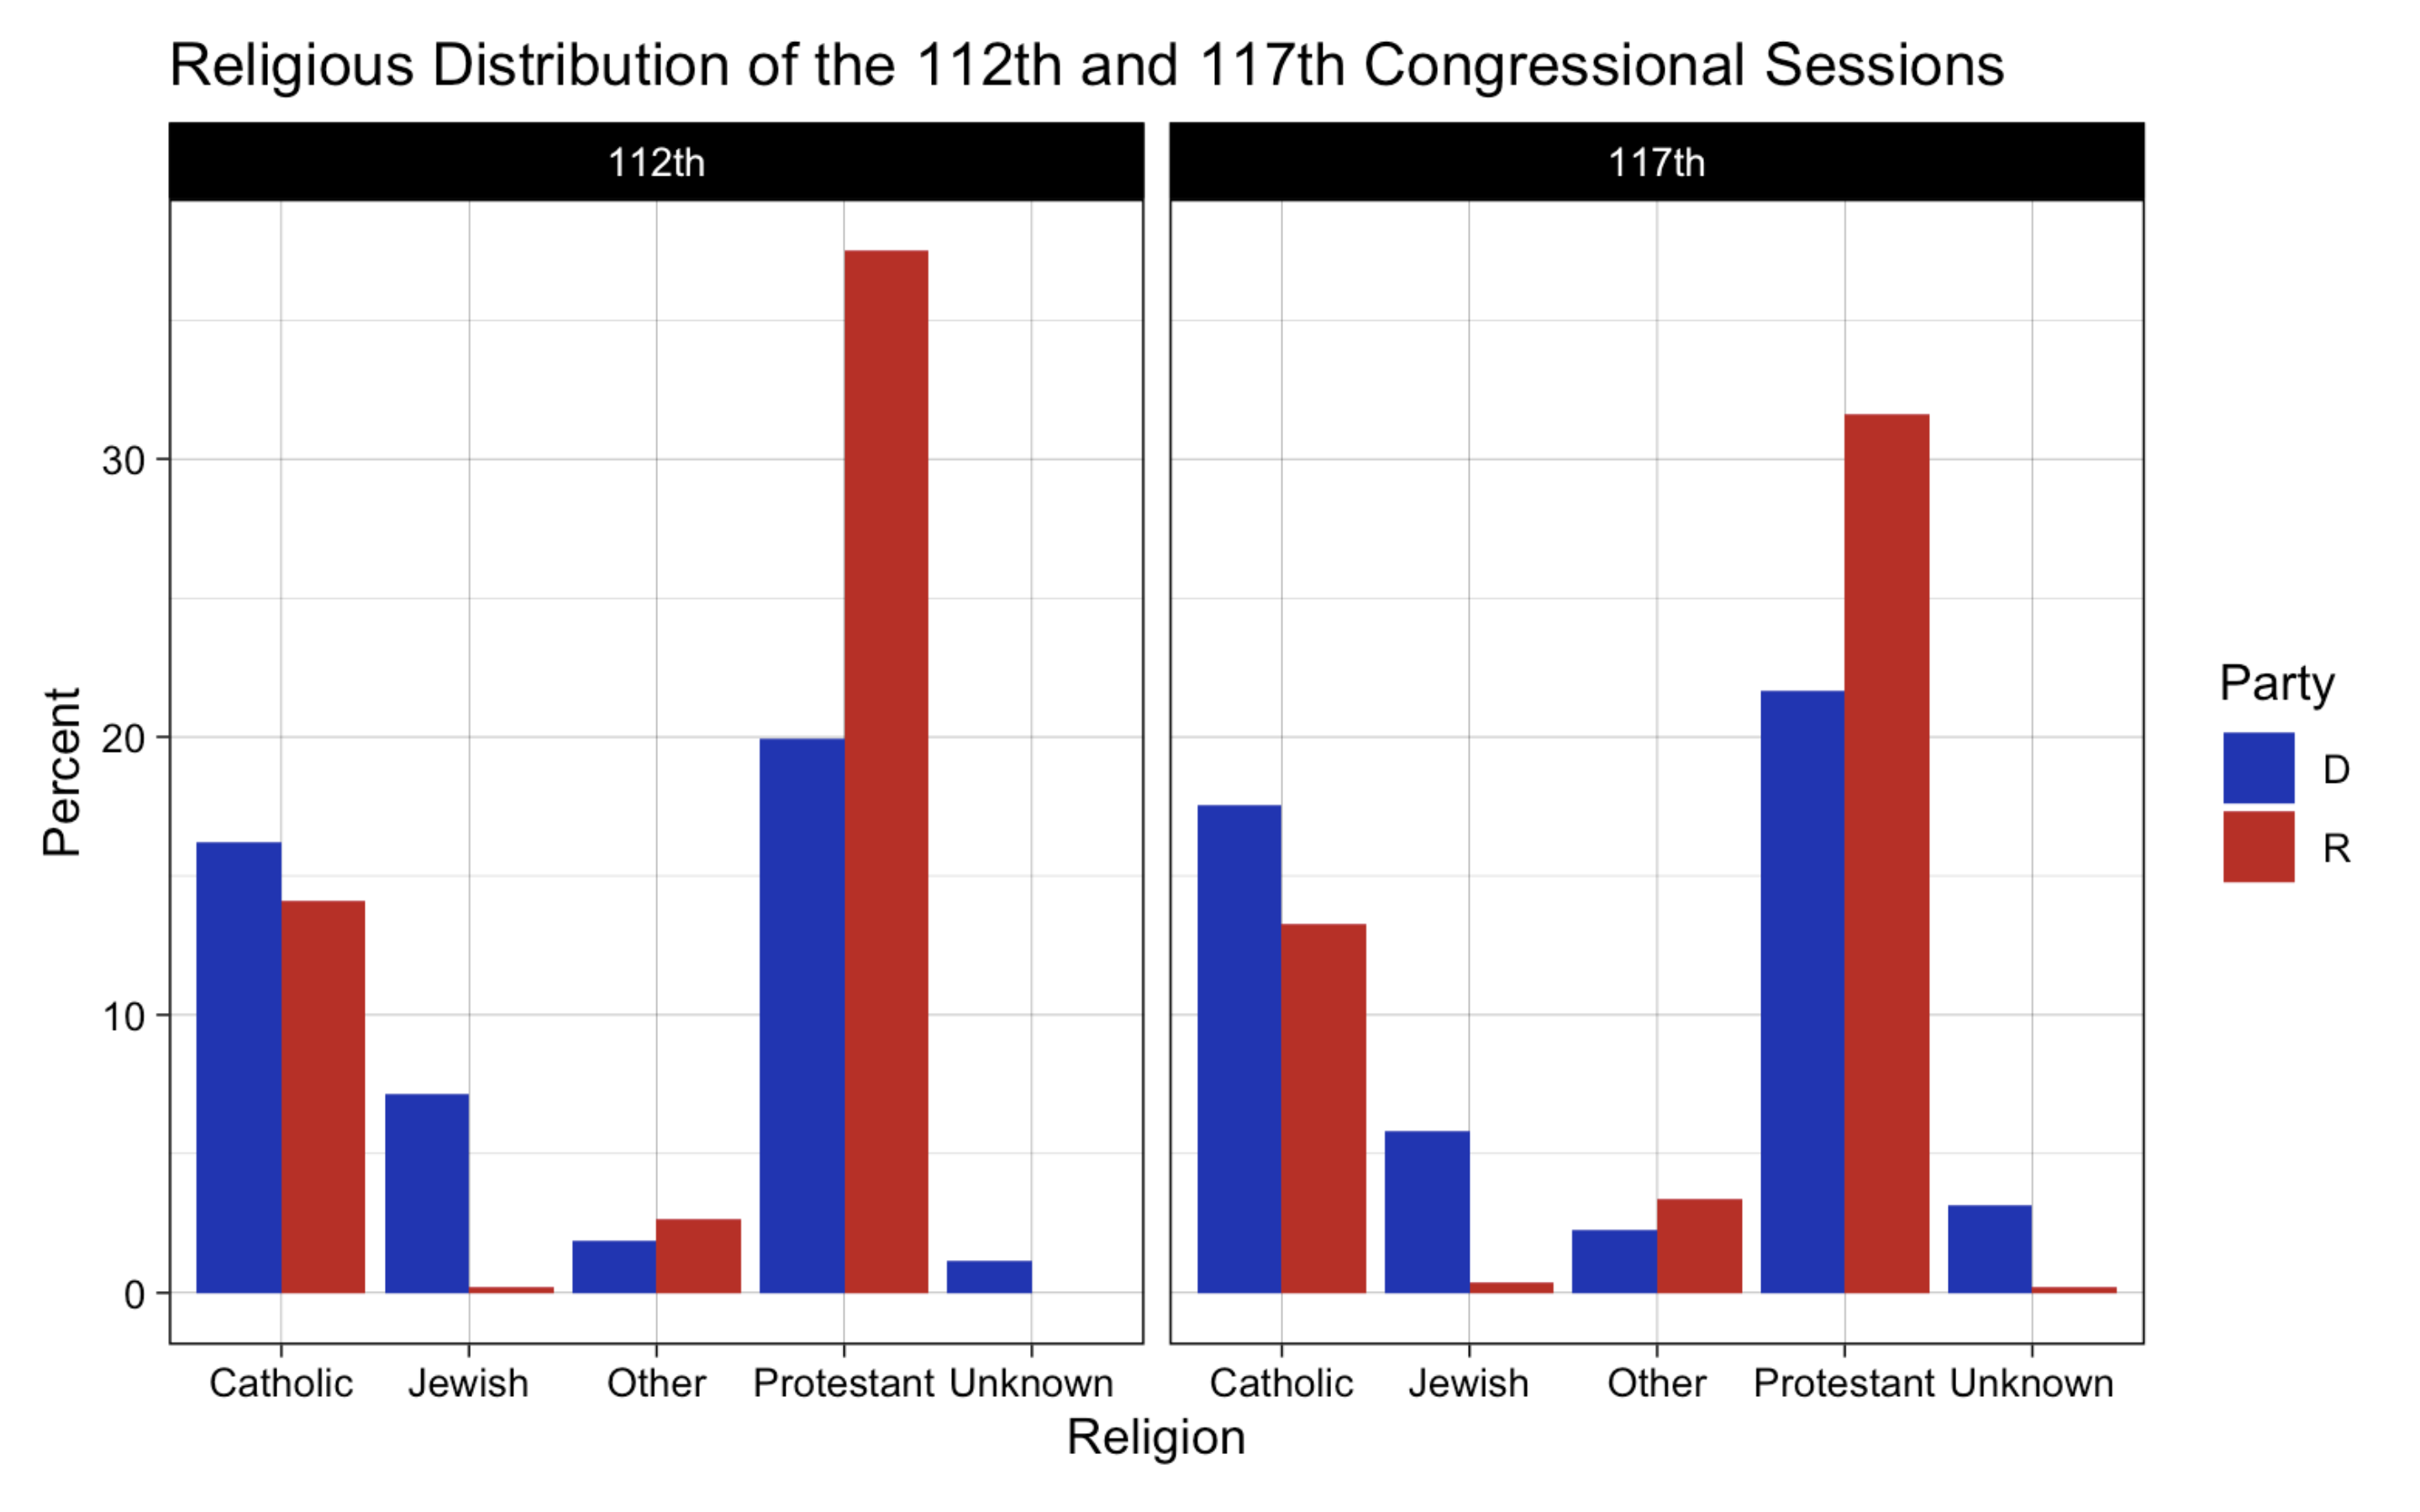
\includegraphics[width=0.95\linewidth]{images/percent_graph} 

}

\caption{Final breakdown for 112th and 117th Congressional sessions after using methodology from the Pew Research Center.\label{fig:figure1}}\label{fig:unnamed-chunk-1}
\end{figure}

For the 112th congress we reduced four of the original religions
affiliations reported--Anglican, Anglican Catholic, Roman Catholic, and
Unitarian--to Catholic. All four of these religions are either Catholic
in and of themselves, follow the same religious beliefs as Catholics, or
are a smaller branch of Catholicism. We then continued this process,
reducing 25 religious affiliations to Protestant, one religious
affiliation to Jewish, six religious affiliations to Other, and two
affiliations to Unknown. The most interesting category is Other with
there being Quakers, Nazarenes, Greek Orthodox, Mormon, Buddhist, and
Muslim. These breakdowns can be seen further in figure
\ref{fig:figure2}.

\begin{figure}

{\centering 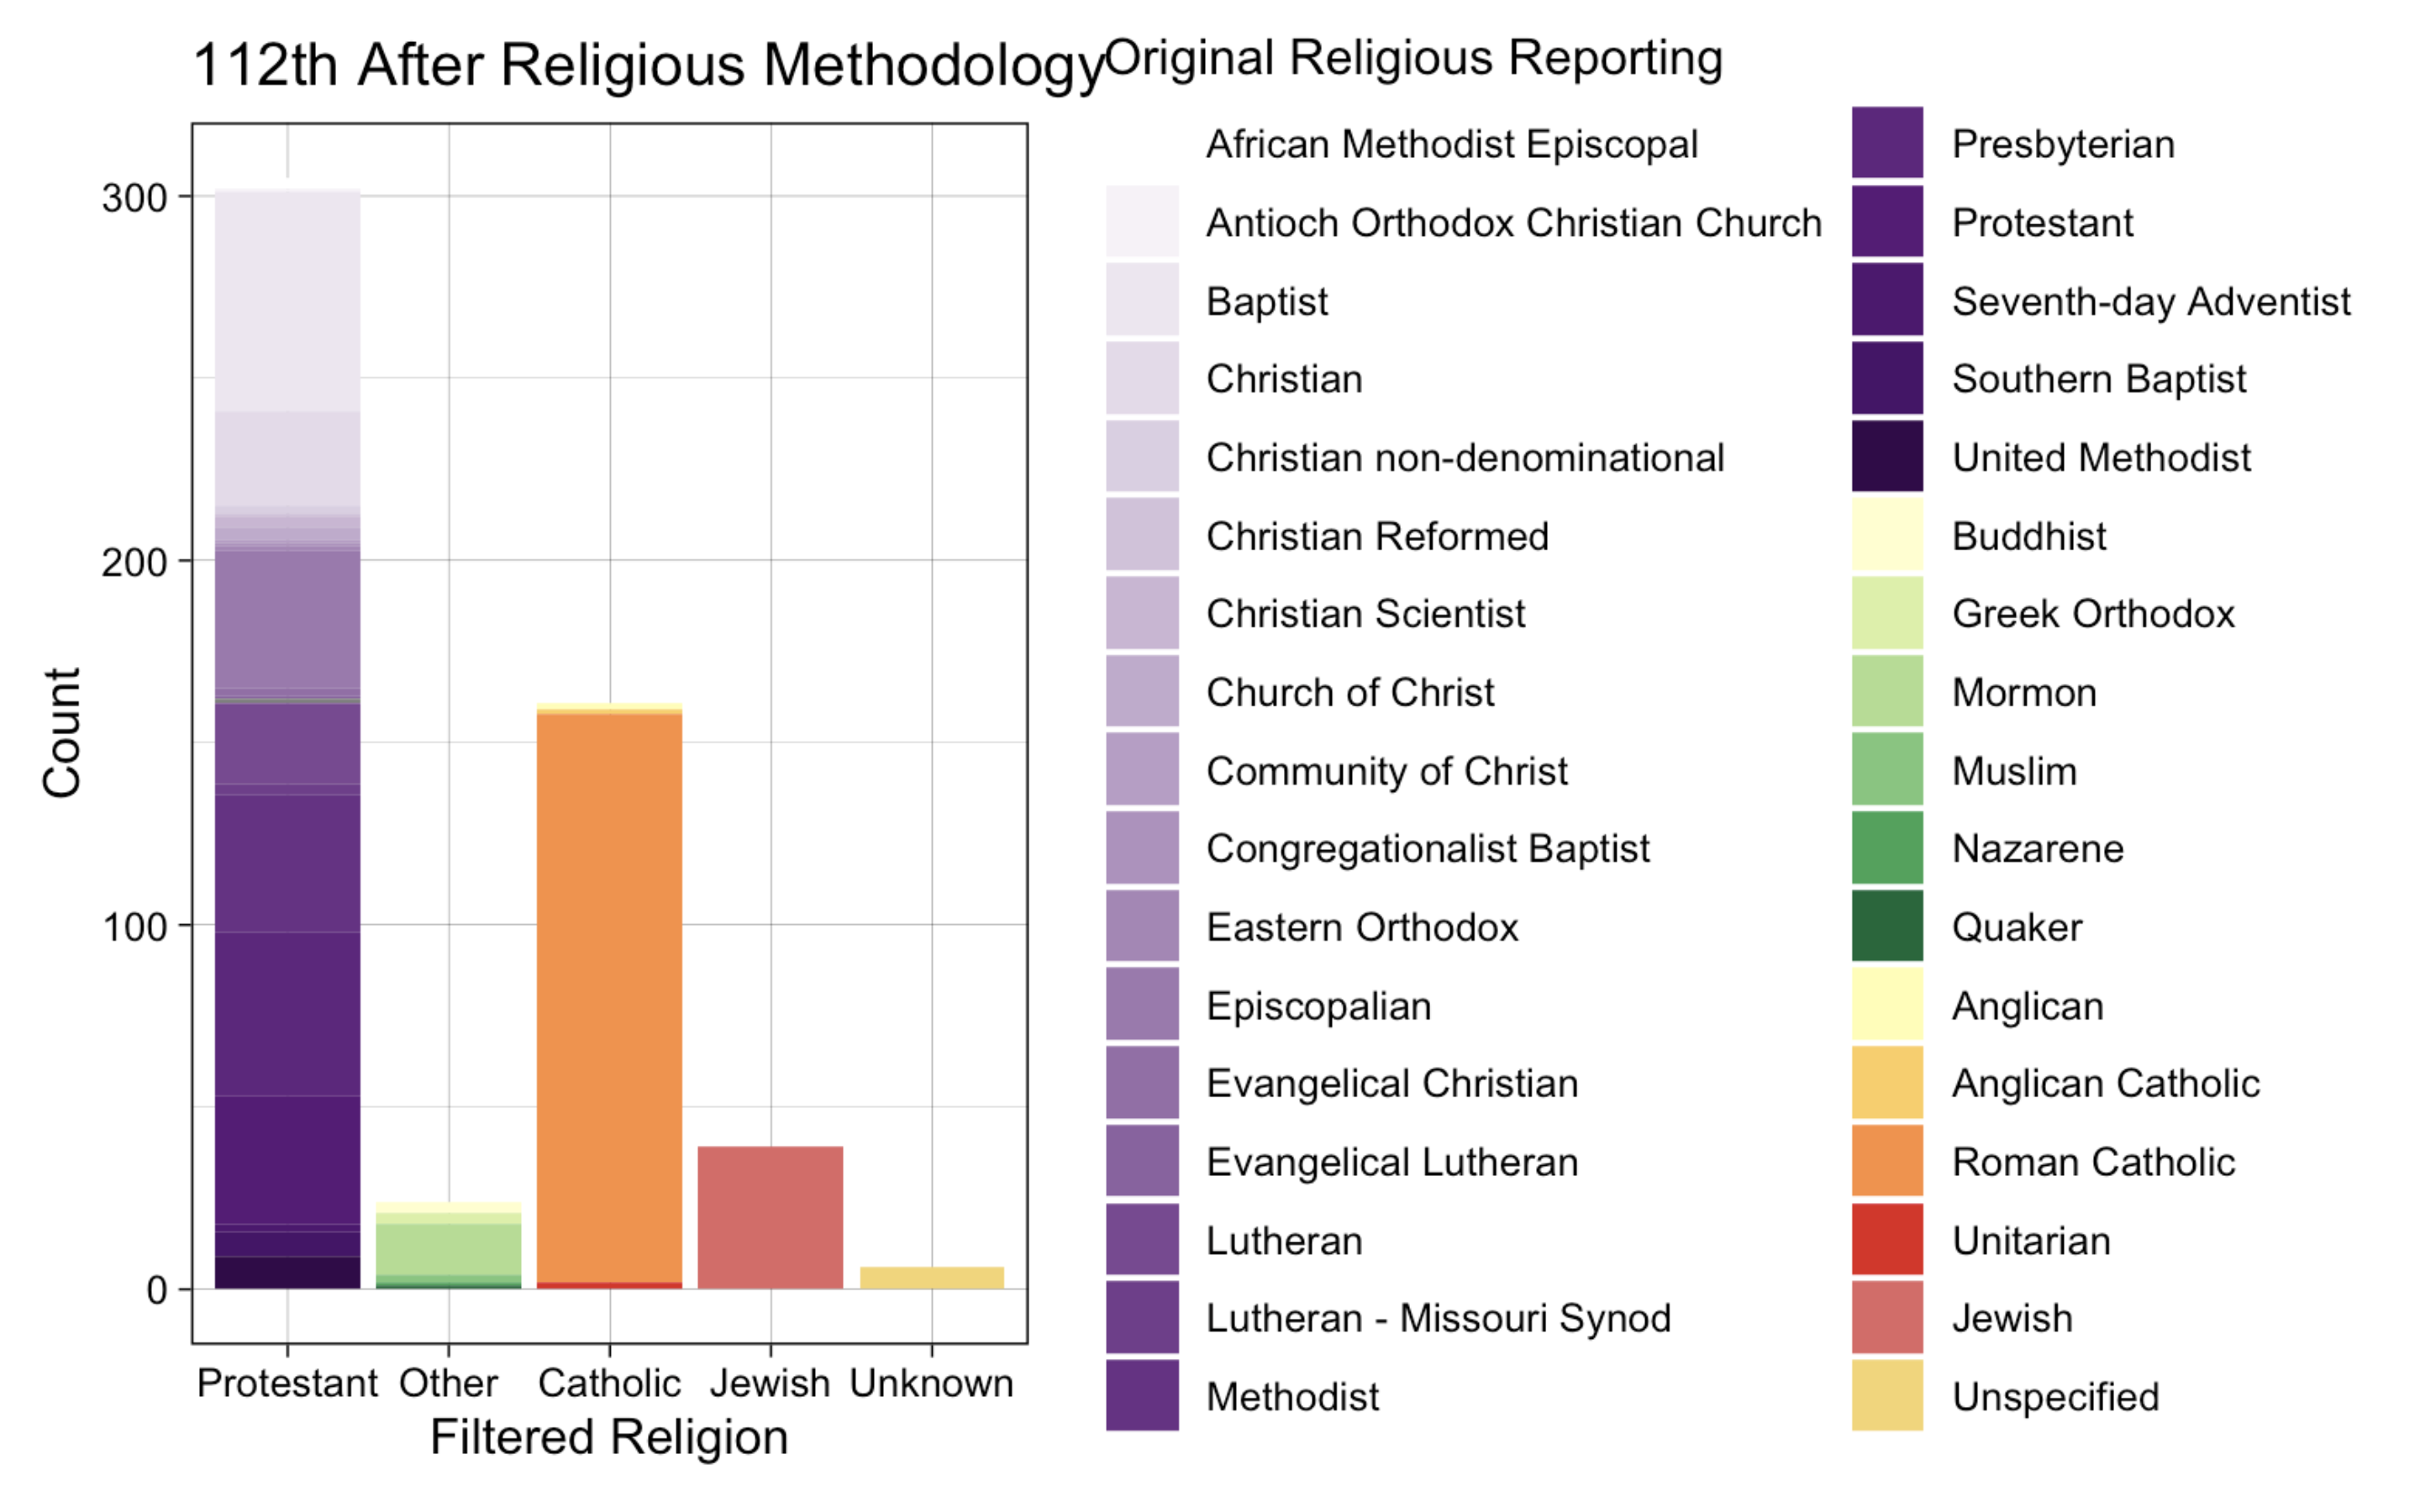
\includegraphics[width=0.95\linewidth]{images/112th_religious} 

}

\caption{Original breakdown of the 112th Congressional session before using methodology from Pew Research Center. Allows for a better understanding of what the origional categorizations were initially.\label{fig:figure2}}\label{fig:unnamed-chunk-2}
\end{figure}

For the 117th congress there were 24 broad religious affiliations. By
using the Pew Research Center's methodology we separated two
affiliations as Catholic, 13 religious affiliations as Protestant, one
as Jewish, six as Other and two as Unknown. The Other category is made
up of Unaffiliated, Buddhist, Hindu, Mormon, Muslim, and
Nondenominational. These breakdowns can be seen further in figure
\ref{fig:figure3}.

Across both sessions of congress when two members belong to the same of
these five groups they are given a 1 and they are given a 0 if they
belong to different groups. Thus this edge level covariable is not
directed, binary, and does not include self ties.

\begin{figure}

{\centering 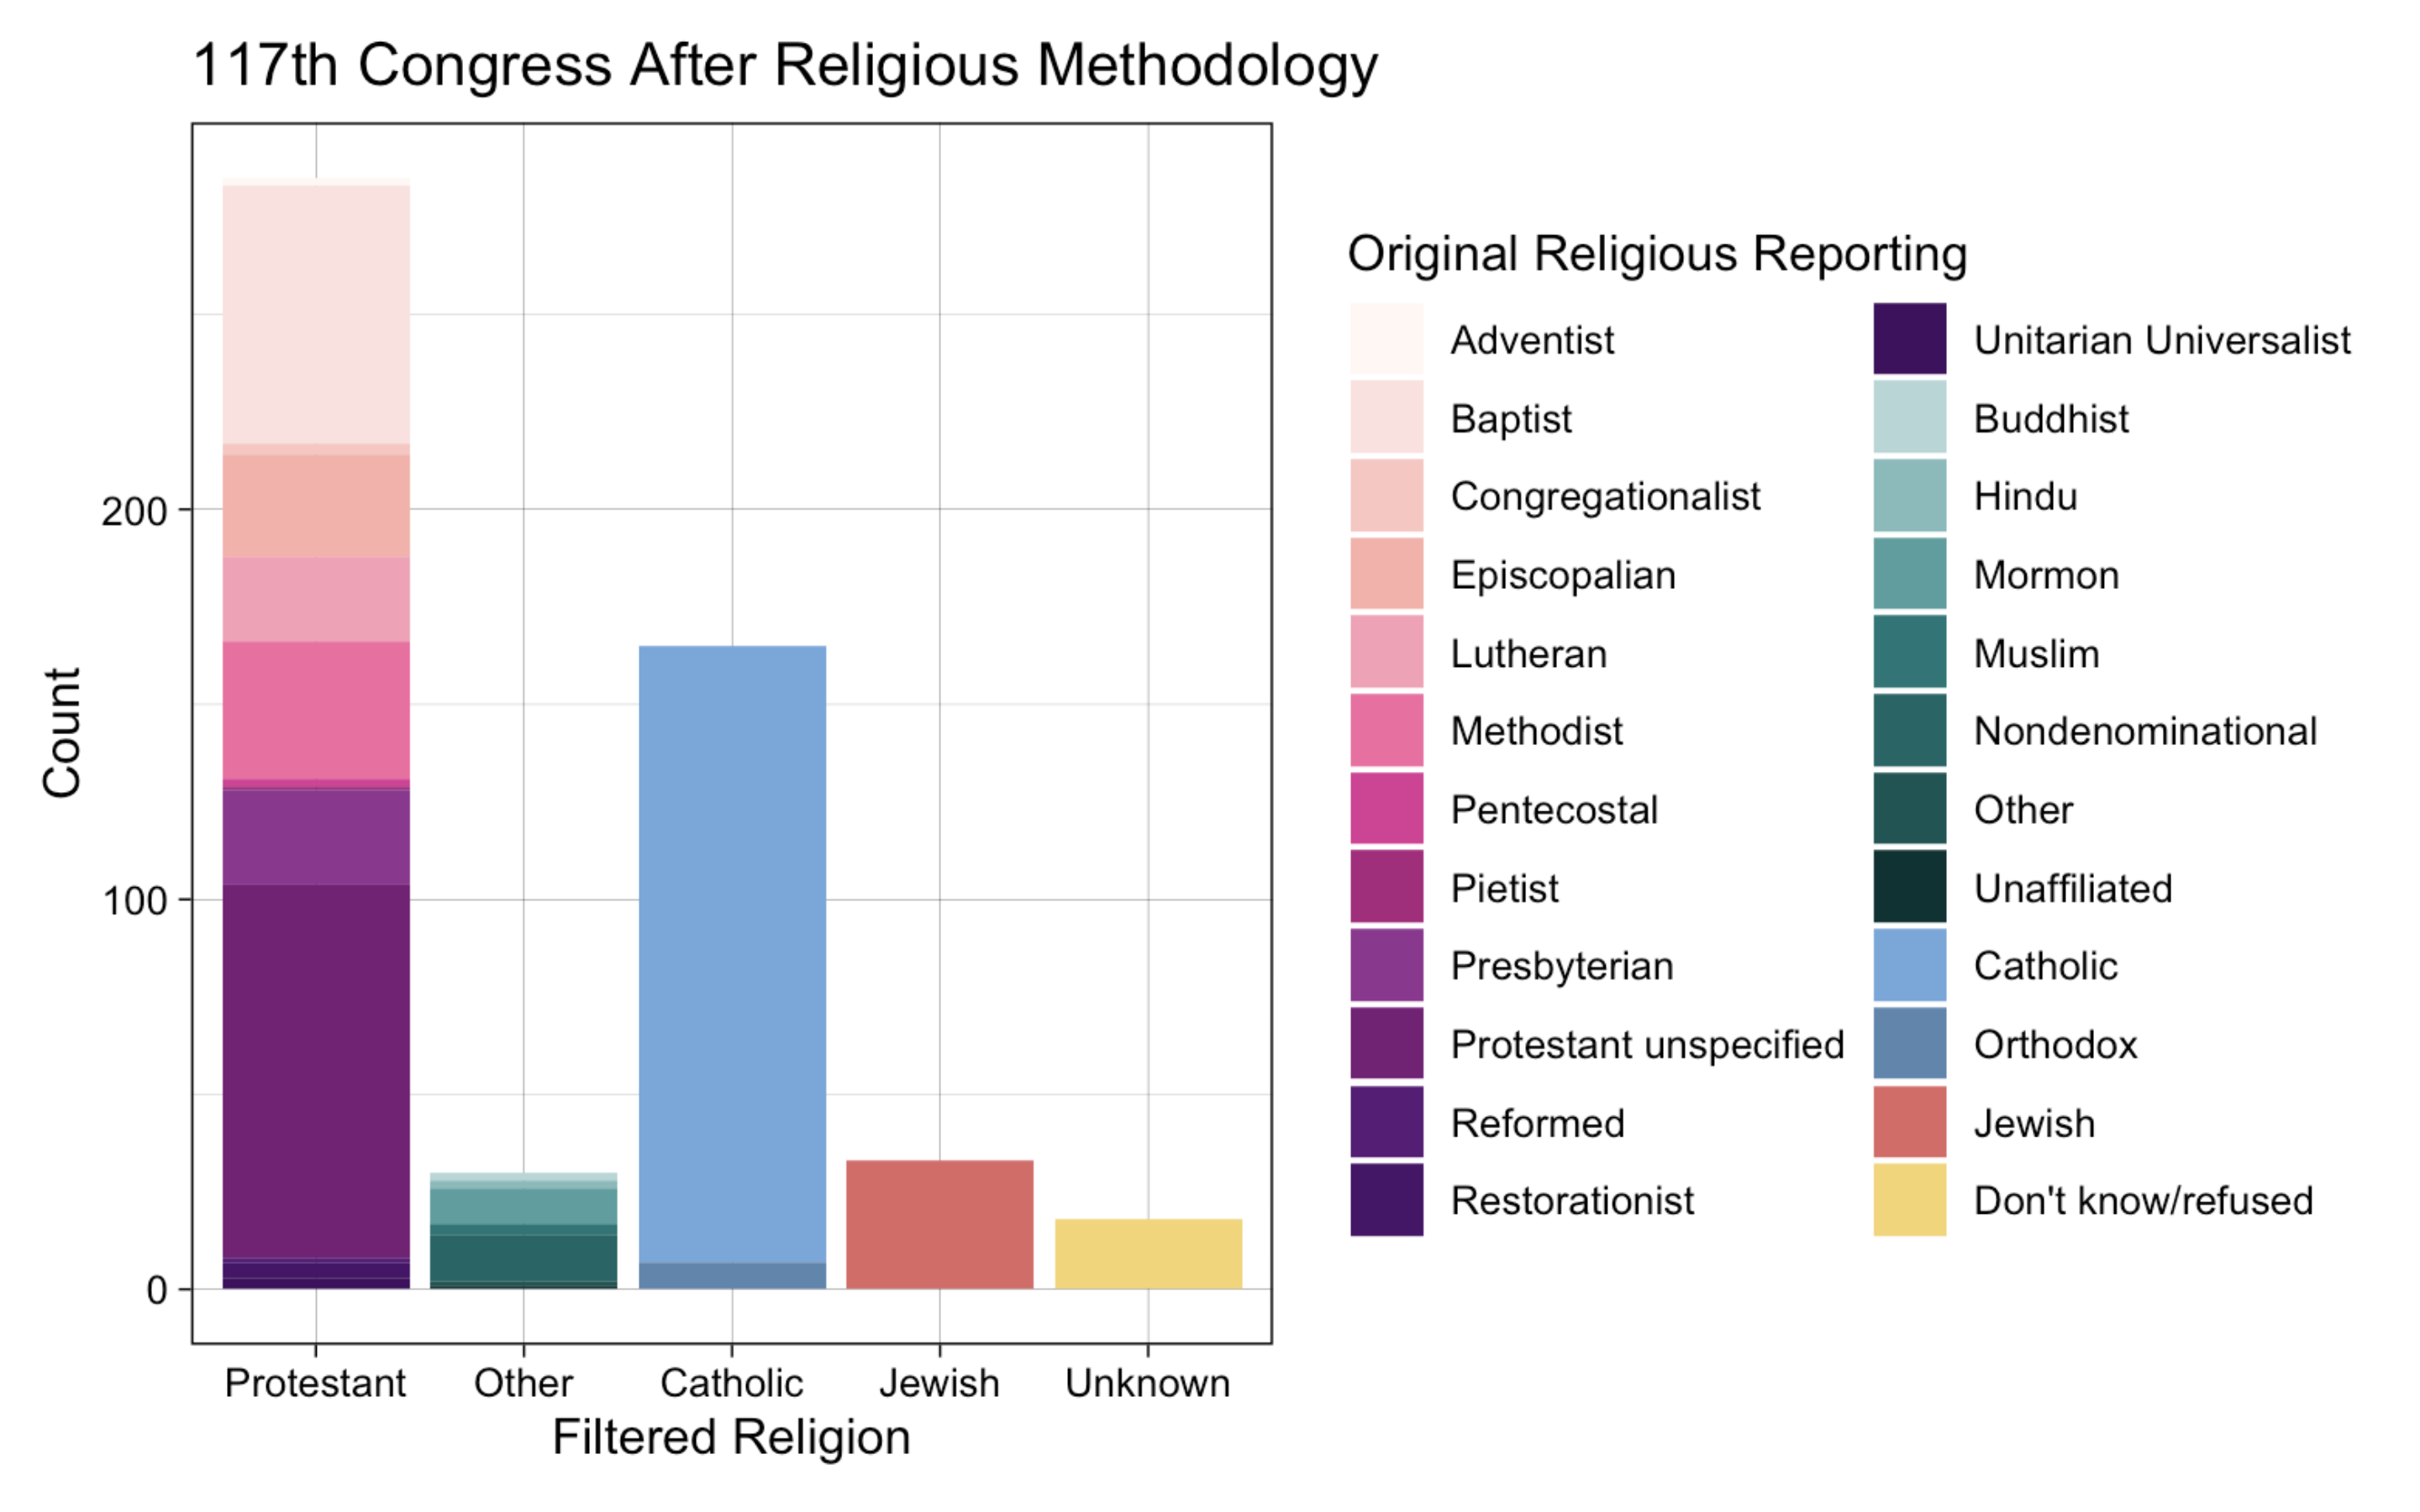
\includegraphics[width=0.85\linewidth]{images/117th religious} 

}

\caption{Original breakdown of the 117th Congressional session before using methodology from Pew Research Center. Allows for a better understanding of what the origional categorizations were initially.\label{fig:figure3}}\label{fig:unnamed-chunk-3}
\end{figure}

\hypertarget{results}{%
\section{Results}\label{results}}

~~Model 1 looks at religious affiliation's effect on cosponsorship for
the 112th and 117th Congress' with the control variables of party and
ideology. The results in figure \ref{fig:figure4} show that for the
112th Congress religious affiliation is not statistically significant,
meaning we have no evidence to suggest that a legislator of the 112th is
more likely to cosponsor legislation with another member of their
religious group after accounting for party and ideology. However, when
looking at the recent 117th we find that religious affiliation is
statistically significant at the .05 alpha level. This means that for
the 117th Congress we have evidence to suggest that legislators are more
likely to cosponsor legislation with someone of the same religious group
after accounting for party and ideology.

\begin{figure}

{\centering 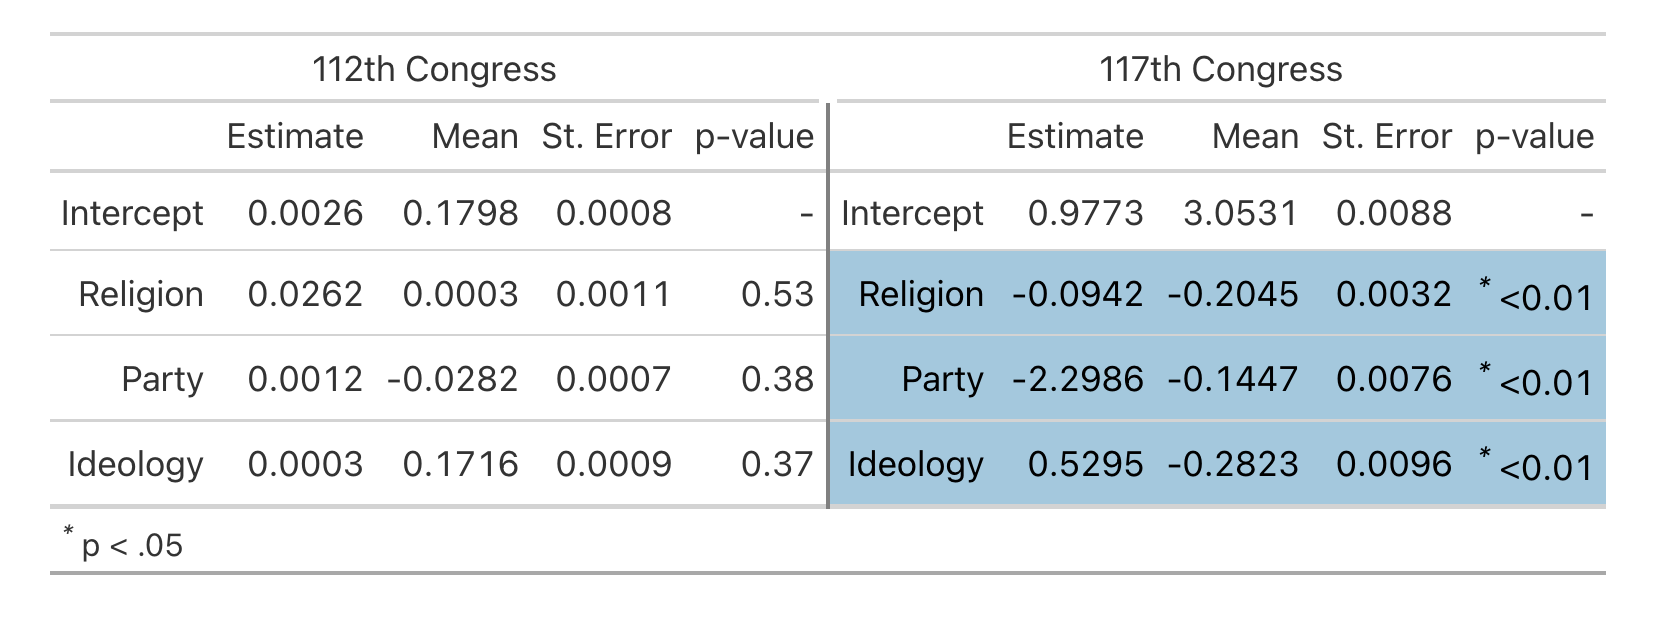
\includegraphics[width=0.85\linewidth]{images/final_model1} 

}

\caption{Model 1 results. Statistically significant rows are highlighted in blue along with stars next to the p-values. \label{fig:figure4}}\label{fig:unnamed-chunk-4}
\end{figure}

This model addresses both our general and polarization hypotheses and
supports both of them. With evidence for our general in the 117th
session, as legislators tend to cosponsor legislation with other members
of their religious group more than with members outside of their
religious group. There is also evidence that polarization along
religious lines has increased between the 112th and 117th congressional
sessions since we find \texttt{religion} to be statistically significant
for only the most recent session.

Model 2 looks at minority group behavior surrounding religion by
modeling the likelihood of each religious group to cosponsor legislation
with other members of their group. Model 3 looks at the same topic
except includes control variables for party and ideology. The results of
these models in figures \ref{fig:figure5} and \ref{fig:figure6}
respectively support part of our hypothesis on minority group behavior.
The results are similar for both models and include three main findings:
Jewish, Protestant, and Unknown are all statistically significant at the
.05 alpha level for the 117th Congress, but nothing is statistically
significant for the 112th.

\begin{figure}

{\centering 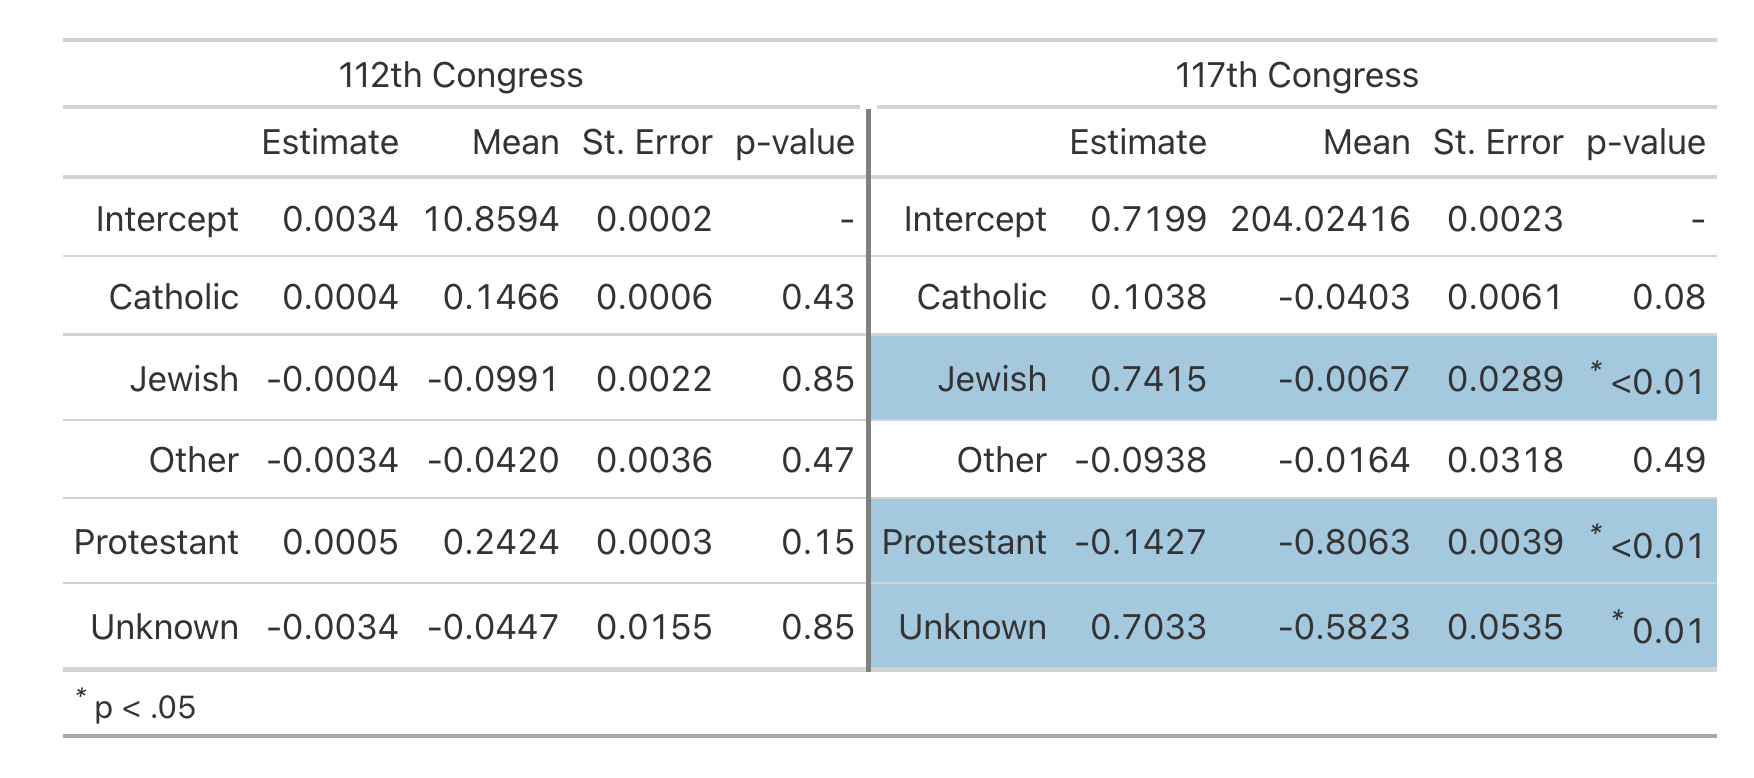
\includegraphics[width=0.85\linewidth]{images/final_model2} 

}

\caption{Results from model 2. Statistically significant results are accompanied by a blue highlighting in the row and a star next to the p-value. \label{fig:figure5}}\label{fig:unnamed-chunk-5}
\end{figure}

This means that Jewish legislators in both the House and Senate are more
likely to cosponsor legislation with other Jewish members, both before
and after accounting for party and ideology. While this finding is
consistent with our second hypothesis on minority group behavior, we
also expected Other to be statistically significant, as this would show
that minority groups such as Muslim or Hindu are more likely to
cosponsor legislation with other Muslims or Hindus respectively. The
next two findings are not consistent with hypothesis 2 as we found
Protestant legislators in the 117th are statistically less likely to
cosponsor legislation with other Protestants both before and after
accounting for party and ideology. Finally we found that Unknown
legislators in the 117th are statistically more likely to cosponsor
legislation with other Unknown legislators. Again these are not very
consistent with our hypotheses as we did not expect Protestants to be
statistically significant as they are not a minority group.

\begin{figure}

{\centering 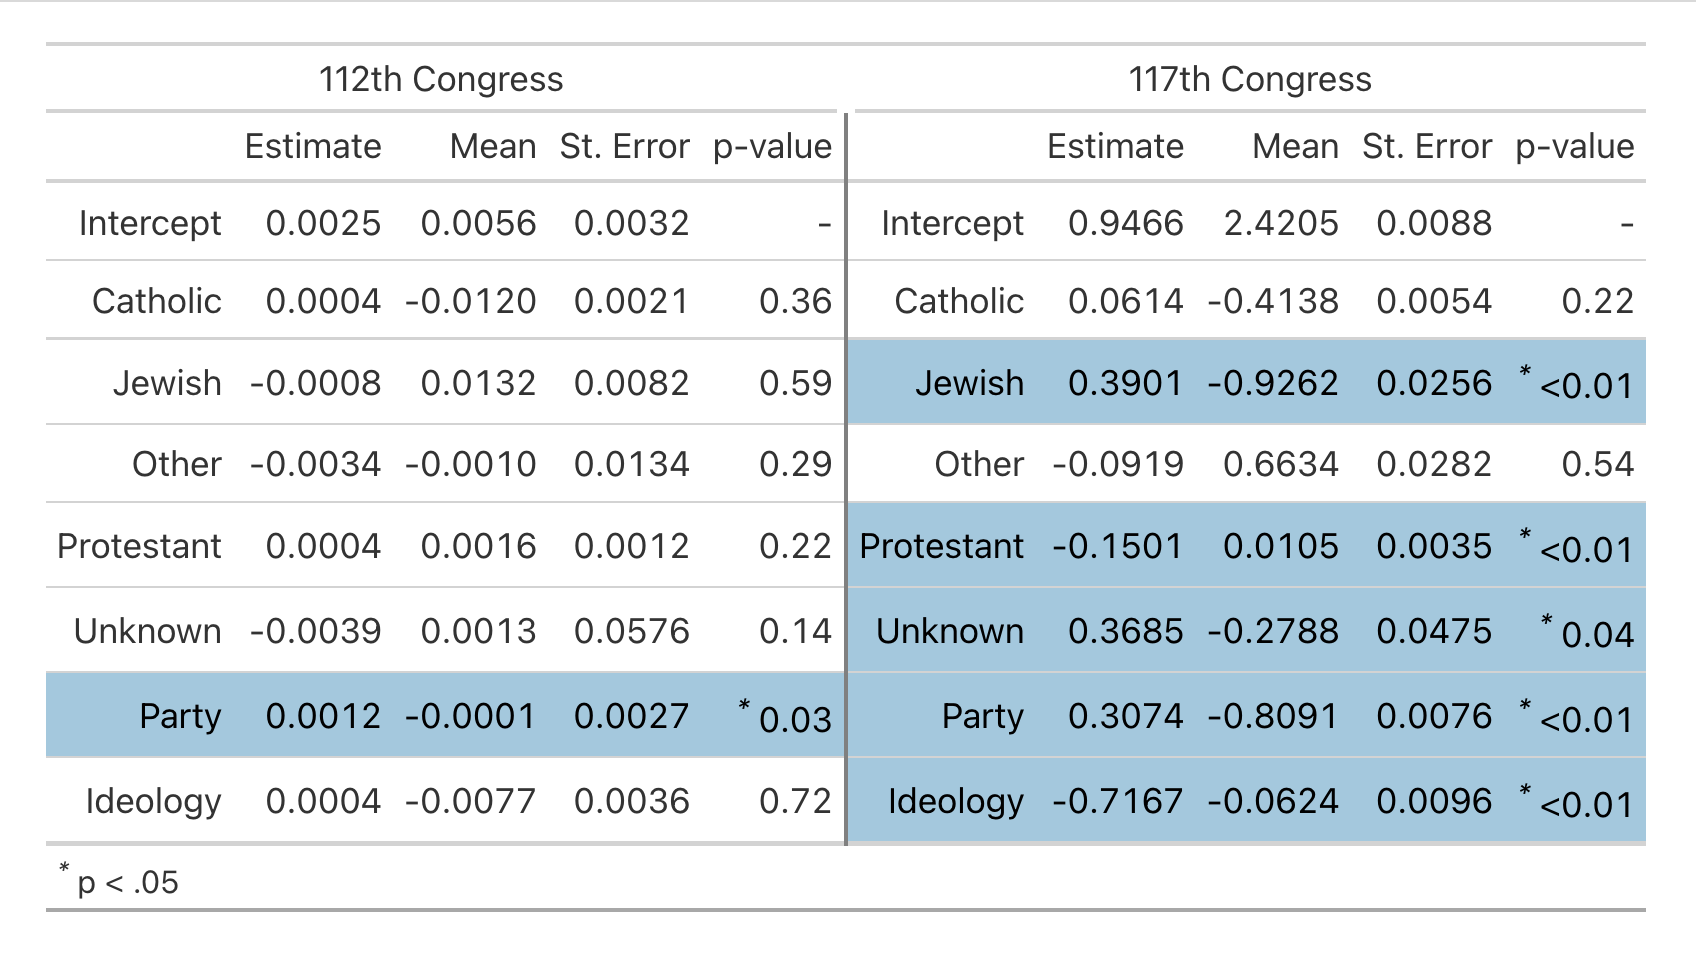
\includegraphics[width=0.85\linewidth]{images/final_model3} 

}

\caption{Results from model 3. Statistically significant results are accompanied by a blue highlighting in the row and a star next to the p-value. \label{fig:figure6}}\label{fig:unnamed-chunk-6}
\end{figure}

However, these findings are consistent with our third polarization
hypothesis as we found no religious groups to be statistically
significant for the 112th Congress, but many for the 117th Congress both
including and excluding control variables identity and party. Thus we
find that there is evidence that religious affiliation plays a part in
cosponsorship in the 117th Congressional session, but not in the 112th.
This suggests the possible increase in polarization from the 112th to
117th sessions.

\hypertarget{conclusion}{%
\section{Conclusion}\label{conclusion}}

~~Our study is the first of its kind, it found a relationship between
the identity-based characteristic of religion and the behaviors of
legislators involved in the congressional cosponsorship network. As
identity-based characteristics have become increasingly politicized and
therefore polarized, it is important to understand its effects on the
congressional network. Research has shown that political identities
(i.e., partisanship and political ideology) and visible identity
characteristics (i.e., age, race, gender) affect the ways in which
legislatures collaborate and contribute to polarization. In this paper,
we have focused on the United States 112th Congress (2011-2013) and the
117th Congress (2021-2023) to understand the effect of religious
affiliation on congressional ties and how that has changed over the past
ten years. This paper pioneers a path for studying religion and
cosponsorship, and provides empirical evidence that the congressional
cosponsorship network is affected by legislators' religious identity.

Given the split result by congressional terms, two major conclusions can
be drawn from this research. First, the network analysis of the 117th
Congress provides evidence that religious affiliation has an effect on
the cosponsorship network. Specifically, this effect is regardless of
minority and majority status as both Jewish and Protestant (minority and
majority groups respectively) are statistically significant.
Practically, this means legislators will be more likely to cosponsor
measures sponsored by colleagues with the same religious affiliation,
but we have little to suggest minority based homophily outside of Jewish
legislators. These findings imply the effects of religion are comparable
to other key identity characteristics as discovered in existing reports
\citep{rocca} .

Secondly, the inconclusive results for the 112th Congress provide
evidence that religion did not have a statistically significant effect
on the cosponsorship network of 2011 to 2013. While this challenges the
general hypothesis that religion would impact the ways in which
legislatures collaborate, it does mean religion's effect on the
congressional network is a relatively new phenomenon. This, in turn,
provides evidence for our third hypothesis, meaning political
polarization based on religion has increased overtime .

There were a few anomalies within our research that are important to
address and suggest solutions for. We expected the `Other' category to
be statistically significant, as those are other minority groups within
Congress and we hypothesized their positive relationship. However,
`Other' includes many different religious groups with drastically
different beliefs such as Mormon and Muslim. It seems incorrect to
expect these religious groups to work together more than others. This is
an excellent place for improvement, as studying specifically these
minority groups against each other could yield positive results.
However, realistically that can not happen until there is wider
representation of minority religions (i.e.~Islam and Mormonism) in
Congress. Extrapolating claims based on one or two legislators is quite
difficult and would present flaws of its own.

While our study is not the first to limit the congressional terms
studies \citep[see][]{bratton2011}, it is important to note when
establishing and making claims about trends. There is always a
possibility these terms are anomalies rather than indicative of the
direction of congress. Future research should focus on the 10 years
between our findings to find the exact shift of religion's influence on
congressional cosponsorship.

Despite these limitations, there are substantial practical implications
of this paper surrounding methodology for studying religion in relation
to cosponsorship in the United States Congress. As the first of its
kind, this paper pioneers a new methodology for studying religion in
network form, and allows further research to be built upon it. Our paper
bridges the gap between existing literature on general cosponsorship and
the effects of identity on congressional behavior. Our paper builds on
both to find religion's influences on the ways legislators collaborate
and therefore collectively build the legislative agenda. This provides a
new avenue of research for future scholars. More notably, this paper
points to the future of congressional politics, eliciting more questions
about the mechanisms that lead to polarization. Further research should
explore, how the greater public is impacted when legislatures are
influenced by religion when deciding what bills gather support?

\bibliographystyle{sageh}
\bibliography{bibfile}


\end{document}
